% !TEX program = pdflatex
% Standalone DynaQGNN ansatz circuit figure.
% Compile: pdflatex fig-dynaqgnn-ansatz.tex  ->  fig-dynaqgnn-ansatz.pdf
% Tuan thu Gem 2 conventions.

\documentclass[tikz,border=10pt]{standalone}

\usepackage[utf8]{inputenc}
\usepackage[T1]{fontenc}
\usepackage{amsmath}
\usepackage{physics}
\usepackage{tikz}
\usepackage{pgfplots}
\pgfplotsset{compat=1.18}

\usetikzlibrary{arrows.meta, positioning, calc, shapes, shapes.geometric,
                fit, backgrounds, shadows.blur, decorations.pathreplacing}

% ===== Palette =====
\definecolor{primary}{RGB}{11, 95, 165}
\definecolor{secondary}{RGB}{184, 134, 11}
\definecolor{success}{RGB}{46, 139, 87}
\definecolor{danger}{RGB}{178, 34, 34}
\definecolor{neutral}{RGB}{96, 106, 115}
\definecolor{encfill}{RGB}{234, 243, 253}
\definecolor{varfill}{RGB}{255, 246, 222}
\definecolor{measfill}{RGB}{230, 245, 233}
\definecolor{clfill}{RGB}{245, 240, 250}

% ===== Styles =====
\tikzset{
  stage/.style={
    draw=neutral, thick, rounded corners=4pt,
    minimum width=2.4cm, minimum height=1.6cm,
    font=\sffamily\small, align=center,
    drop shadow={blur shadow={shadow xshift=0.5pt, shadow yshift=-0.5pt}}
  },
  enc/.style={stage, fill=encfill, draw=primary},
  var/.style={stage, fill=varfill, draw=secondary},
  meas/.style={stage, fill=measfill, draw=success},
  classical/.style={stage, fill=clfill, draw=neutral},
  data/.style={
    draw=neutral!60, thick, fill=white, shape=cylinder, shape border rotate=90,
    minimum width=1.8cm, minimum height=1.2cm, aspect=0.3,
    font=\sffamily\small, align=center
  },
  flow/.style={-Stealth, very thick, neutral},
  qline/.style={thick, neutral!80},
  gate/.style={draw=primary, thick, fill=primary!15, rounded corners=1pt,
               minimum size=0.55cm, font=\sffamily\tiny\bfseries, inner sep=1pt},
  gatey/.style={draw=secondary, thick, fill=secondary!15, rounded corners=1pt,
               minimum size=0.55cm, font=\sffamily\tiny\bfseries, inner sep=1pt},
  cgate/.style={draw=neutral, fill=neutral!20, circle, minimum size=0.22cm, inner sep=0pt},
  xgate/.style={draw=neutral, fill=white, circle, minimum size=0.32cm, inner sep=0pt,
                label={center:{\tiny $\oplus$}}},
  measg/.style={draw=success, thick, fill=success!15, minimum size=0.6cm,
                font=\sffamily\tiny\bfseries, inner sep=1pt},
  layerlabel/.style={font=\sffamily\footnotesize\itshape, neutral},
}

\begin{document}
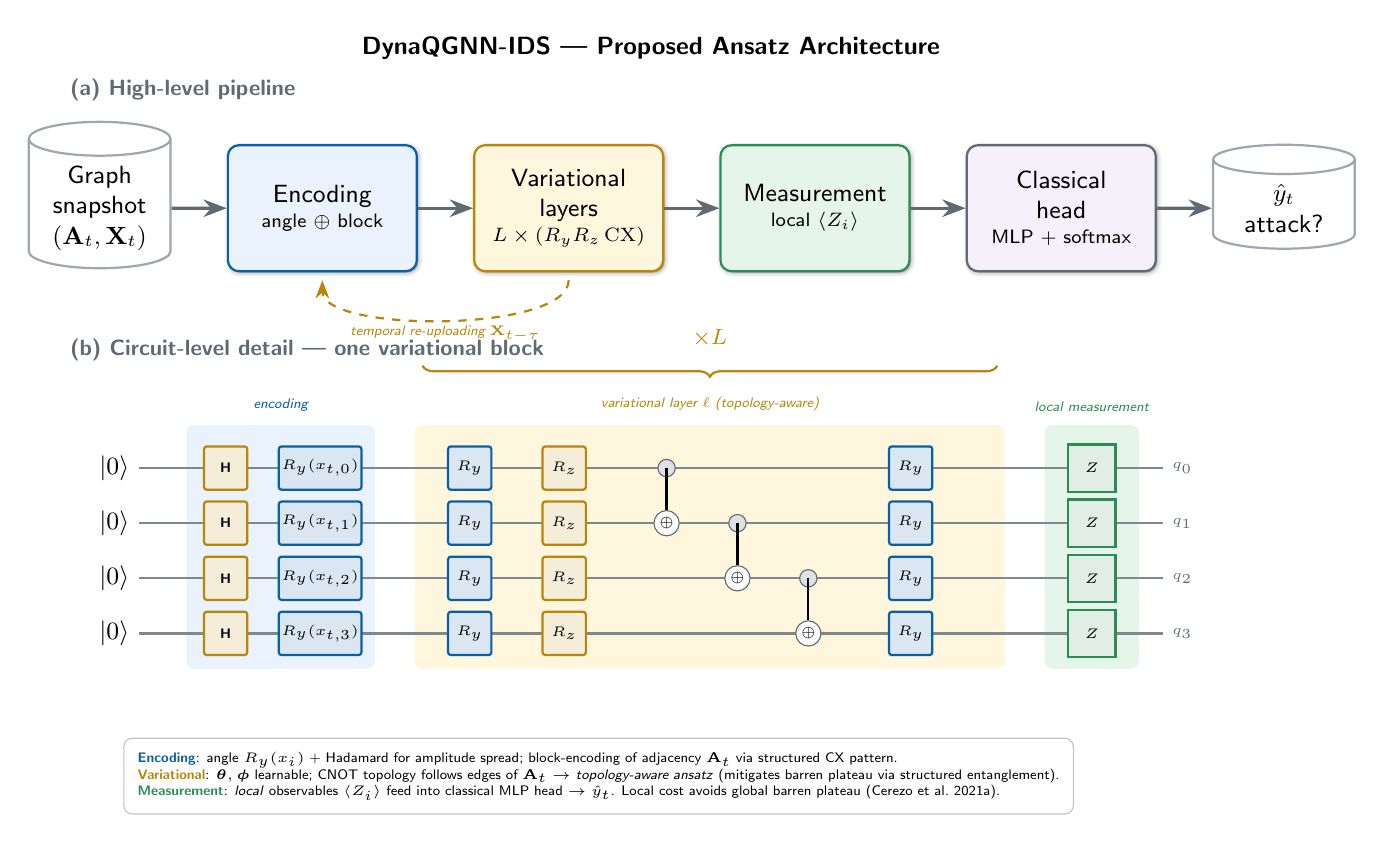
\begin{tikzpicture}[node distance=1cm]

  % ======================================================
  %  HIGH-LEVEL PIPELINE  (top row)
  % ======================================================
  \node[layerlabel, anchor=west] at (-0.5, 4.5)
    {\textbf{(a) High-level pipeline}};

  \node[data] (gs)
    at (0, 3) {Graph\\ snapshot\\ $(\mathbf{A}_t, \mathbf{X}_t)$};

  \node[enc, right=0.7cm of gs] (enc) {Encoding\\[-2pt]\scriptsize angle $\oplus$ block};
  \node[var, right=0.7cm of enc]  (var) {Variational\\ layers\\[-2pt]\scriptsize $L \times (R_y R_z \, \mathrm{CX})$};
  \node[meas, right=0.7cm of var] (meas) {Measurement\\[-2pt]\scriptsize local $\langle Z_i \rangle$};
  \node[classical, right=0.7cm of meas] (cl) {Classical\\ head\\[-2pt]\scriptsize MLP + softmax};
  \node[data, right=0.7cm of cl] (out) {$\hat{y}_t$\\ attack?};

  % Flow arrows
  \draw[flow] (gs)   -- (enc);
  \draw[flow] (enc)  -- (var);
  \draw[flow] (var)  -- (meas);
  \draw[flow] (meas) -- (cl);
  \draw[flow] (cl)   -- (out);

  % Temporal re-uploading loopback (routed BELOW the pipeline to avoid title).
  \draw[-Stealth, thick, dashed, secondary]
    ($(var.south) + (0, -0.1)$) to[out=-90, in=-90, looseness=0.55]
    ($(enc.south) + (0, -0.1)$);
  \node[font=\sffamily\tiny\itshape, secondary, anchor=north]
    at ($(enc.south)!0.5!(var.south) + (0, -0.55)$)
    {temporal re-uploading $\mathbf{X}_{t-\tau}$};

  % ======================================================
  %  CIRCUIT-LEVEL DETAIL  (bottom row)
  % ======================================================
  \node[layerlabel, anchor=west] at (-0.5, 1.2)
    {\textbf{(b) Circuit-level detail --- one variational block}};

  % x-coordinates for circuit
  \def\xstart{0.5}
  \def\xend{13.5}

  % 4 qubit lines
  \foreach \i/\y in {0/-0.3, 1/-1.0, 2/-1.7, 3/-2.4} {
    \draw[qline] (\xstart, \y) -- (\xend, \y);
    \node[anchor=east, font=\sffamily\small] at (\xstart, \y) {$\ket{0}$};
    \node[anchor=west, font=\sffamily\tiny, neutral] at (\xend, \y) {$q_{\i}$};
  }

  % ---------- Encoding block ----------
  \begin{scope}[on background layer]
    \fill[encfill, rounded corners=3pt] (1.1, -2.85) rectangle (3.5, 0.25);
  \end{scope}
  \node[font=\sffamily\tiny\itshape, primary, anchor=south] at (2.3, 0.3) {encoding};

  \foreach \i/\y/\t in {0/-0.3/{x_{t,0}}, 1/-1.0/{x_{t,1}}, 2/-1.7/{x_{t,2}}, 3/-2.4/{x_{t,3}}} {
    \node[gatey] at (1.6, \y) {H};
    \node[gate] at (2.8, \y) {$R_y(\t)$};
  }

  % ---------- Variational block (repeated L times) ----------
  \begin{scope}[on background layer]
    \fill[varfill, rounded corners=3pt] (4.0, -2.85) rectangle (11.5, 0.25);
  \end{scope}
  \node[font=\sffamily\tiny\itshape, secondary, anchor=south] at (7.75, 0.3)
    {variational layer $\ell$ (topology-aware)};

  % Ry rotations
  \foreach \i/\y/\t in {0/-0.3/\theta_{0}^{(\ell)}, 1/-1.0/\theta_{1}^{(\ell)},
                        2/-1.7/\theta_{2}^{(\ell)}, 3/-2.4/\theta_{3}^{(\ell)}} {
    \node[gate]  at (4.7, \y) {$R_y$};
    \node[gatey] at (5.9, \y) {$R_z$};
  }

  % CNOT entangling layer (following adjacency A_t)
  % CNOT: q0 control, q1 target
  \node[cgate] (c01) at (7.2, -0.3) {};
  \node[xgate] (x01) at (7.2, -1.0) {};
  \draw[thick] (c01.center) -- (x01.north);

  % CNOT: q1 control, q2 target
  \node[cgate] (c12) at (8.1, -1.0) {};
  \node[xgate] (x12) at (8.1, -1.7) {};
  \draw[thick] (c12.center) -- (x12.north);

  % CNOT: q2 control, q3 target
  \node[cgate] (c23) at (9.0, -1.7) {};
  \node[xgate] (x23) at (9.0, -2.4) {};
  \draw[thick] (c23.center) -- (x23.north);

  % Second Ry layer
  \foreach \i/\y/\t in {0/-0.3/\phi_{0}^{(\ell)}, 1/-1.0/\phi_{1}^{(\ell)},
                        2/-1.7/\phi_{2}^{(\ell)}, 3/-2.4/\phi_{3}^{(\ell)}} {
    \node[gate]  at (10.3, \y) {$R_y$};
  }

  % ---------- Measurement block ----------
  \begin{scope}[on background layer]
    \fill[measfill, rounded corners=3pt] (12.0, -2.85) rectangle (13.2, 0.25);
  \end{scope}
  \node[font=\sffamily\tiny\itshape, success, anchor=south] at (12.6, 0.3)
    {local measurement};

  \foreach \i/\y in {0/-0.3, 1/-1.0, 2/-1.7, 3/-2.4} {
    \node[measg] at (12.6, \y) {$Z$};
  }

  % Bracket above variational block showing repetition.
  % Placed at y=1.0 with text on top, well clear of the "variational layer" label at y=0.3.
  \draw [decorate,decoration={brace,amplitude=4pt}, thick, secondary]
    (11.4, 1.0) -- (4.1, 1.0)
    node[midway, above=3pt, font=\sffamily\footnotesize\itshape, secondary]
    {$\times L$};

  % ======================================================
  %  ANNOTATIONS (right side)
  % ======================================================
  \node[draw=neutral!40, fill=white, rounded corners=3pt, inner sep=5pt,
        anchor=south west, font=\sffamily\tiny, align=left]
        at (0.3, -4.7) {
    \textcolor{primary}{\textbf{Encoding}}: angle $R_y(x_i)$ + Hadamard for amplitude spread;
    block-encoding of adjacency $\mathbf{A}_t$ via structured CX pattern. \\
    \textcolor{secondary}{\textbf{Variational}}: $\boldsymbol{\theta}, \boldsymbol{\phi}$ learnable;
    CNOT topology follows edges of $\mathbf{A}_t$ $\rightarrow$ \emph{topology-aware ansatz}
    (mitigates barren plateau via structured entanglement). \\
    \textcolor{success}{\textbf{Measurement}}: \emph{local} observables $\langle Z_i \rangle$
    feed into classical MLP head $\rightarrow$ $\hat{y}_t$. Local cost avoids global
    barren plateau (Cerezo et al.\ 2021a).
  };

  % Title (placed higher to clear the re-uploading arc and its label)
  \node[font=\sffamily\small\bfseries, anchor=north, align=center]
    at (7, 5.3) {DynaQGNN-IDS --- Proposed Ansatz Architecture};

\end{tikzpicture}
\end{document}
